% !TeX encoding = ISO-8859-1
% !TeX spellcheck = pt_BR
% Thesis Appendix -------------------------------------------------------

\chapter{Algoritmos Baseados na Grafost�tica}\label{Apend1}

\section{Algoritmo de Soma de Vetores e C�lculo da Equilibrante}
\label{Apend1:somavetconcorre}

\begin{figure}[H]
\begin{center}
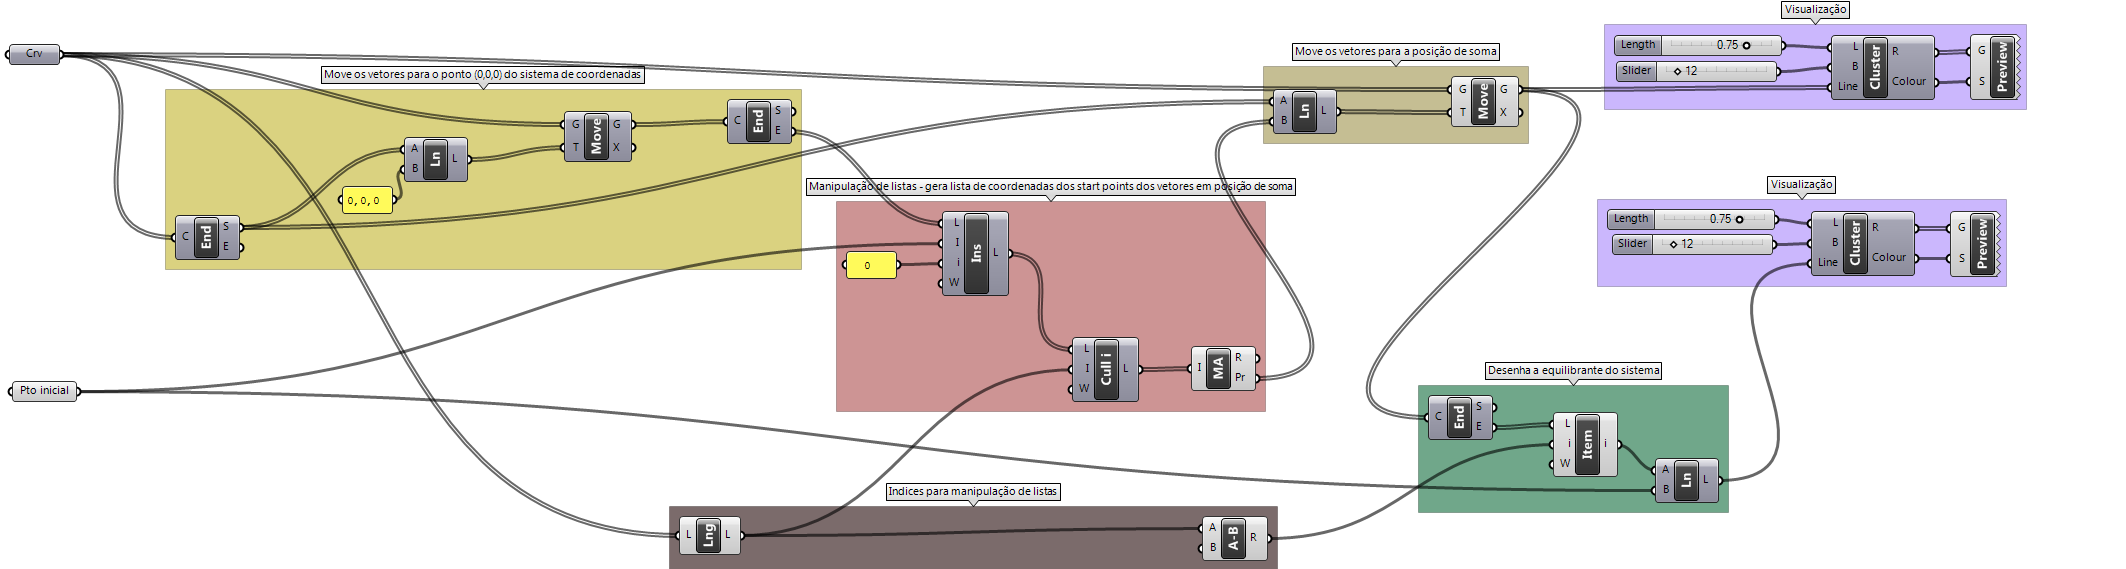
\includegraphics[width=1\textwidth]{SomaDeVetoresConcorrentes.png}
\caption{Captura de Tela do Algoritmo de Soma de Vetores} \label{figura:Ap1:SomaDeVetoresConcorrentes}
\end{center}
\end{figure}


\section{\textit{Cluster} Utilizado para a Visualiza��o de Vetores}
\label{Apend1:clusterVisu}

\begin{figure}[H]
\begin{center}
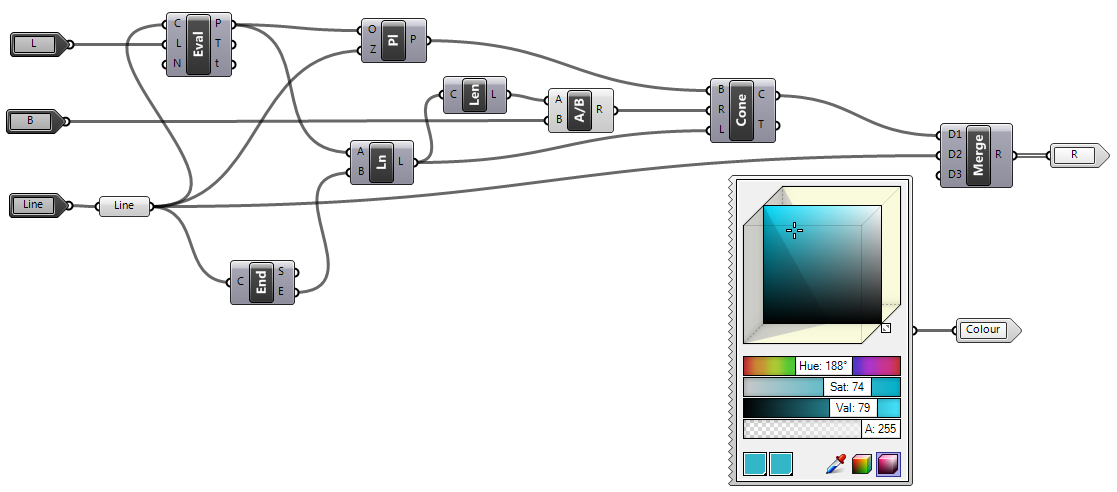
\includegraphics[width=1\textwidth]{clusterVisu.png}
\caption{Captura de Tela do Algoritmo do Cluster de Visualiza��o de Vetores} \label{figura:Ap1:clusterVisu}
\end{center}
\end{figure}



\section{Algoritmo de Desenho do PF, FG, Funicular e C�lculo da Resultante e Momento }
\label{Apend1:funicular1}


\begin{figure}[H]
\begin{center}
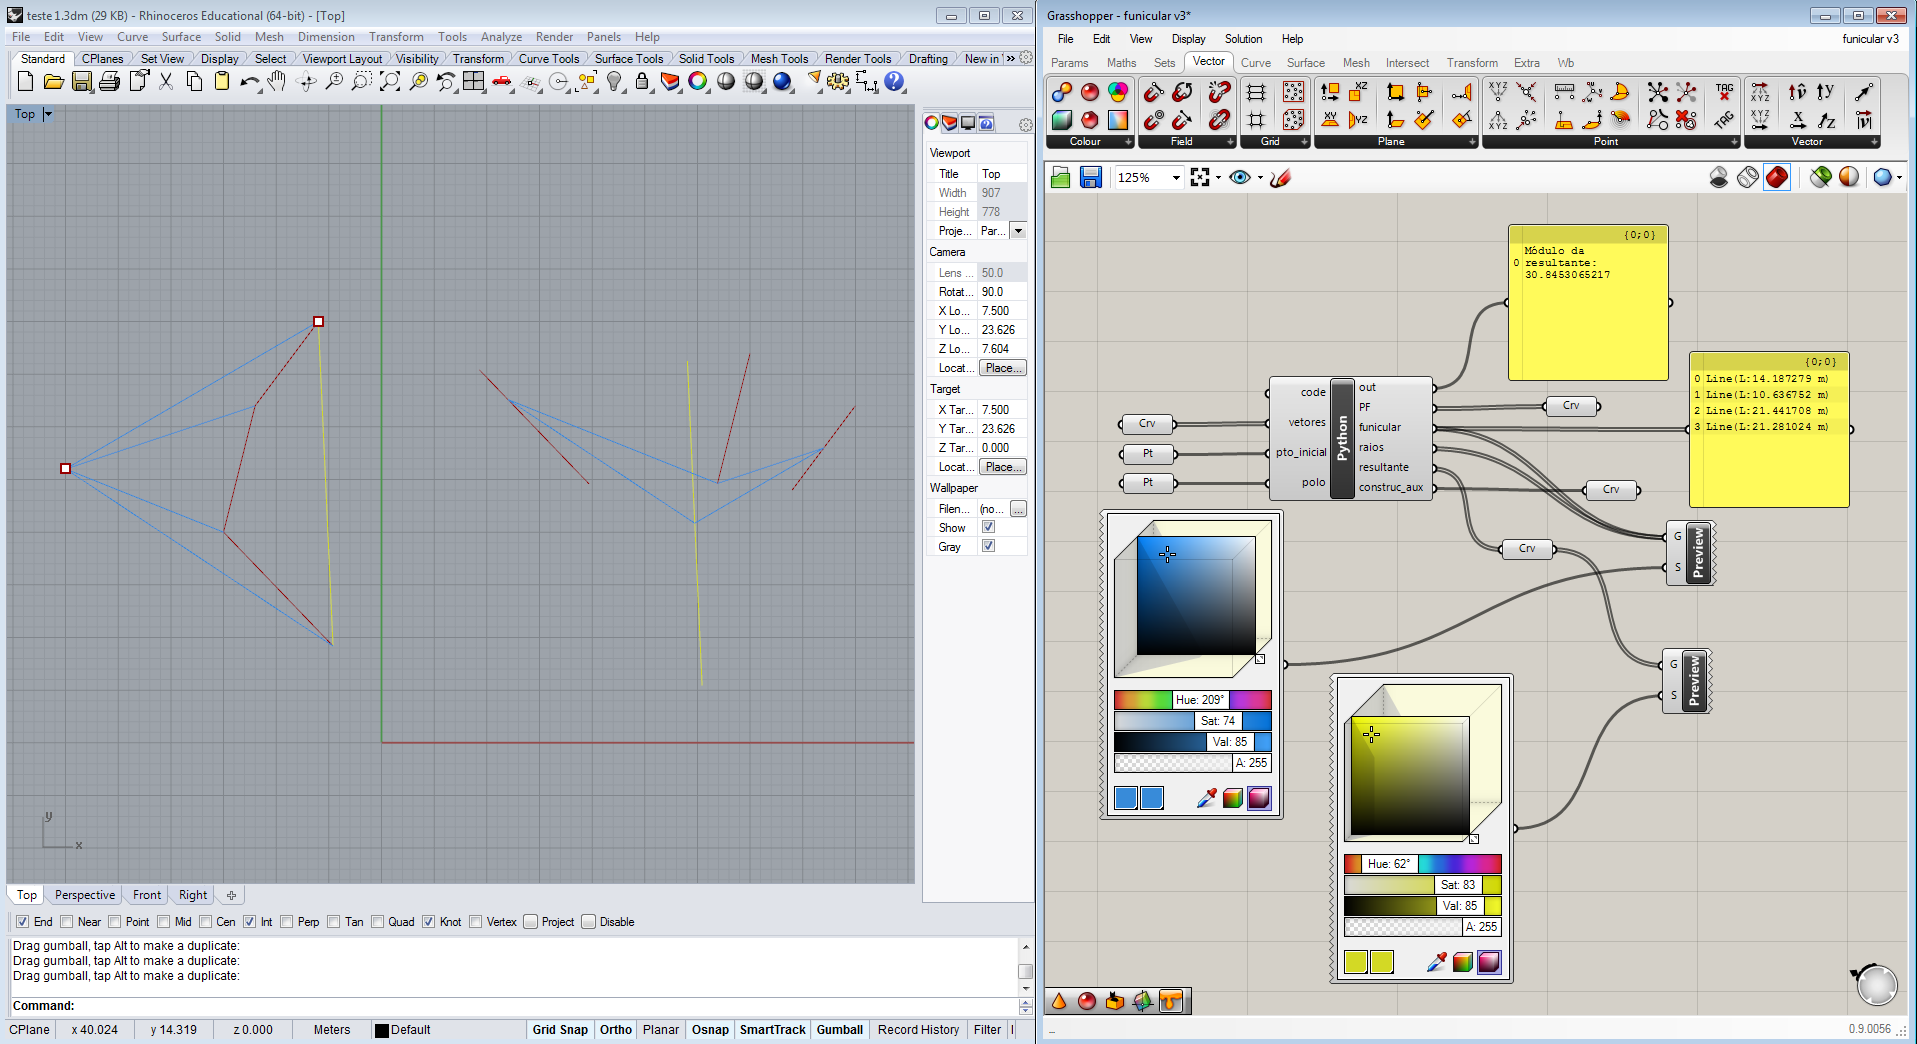
\includegraphics[width=1\textwidth]{Algfunicular01.png}
\caption{Captura de Tela do Algoritmo de Desenho do PF, FG, Funicular, Resultante e Momento} \label{figura:Ap1:Algfunicular01}
\end{center}
\end{figure}

\begin{figure}[H]
\begin{center}
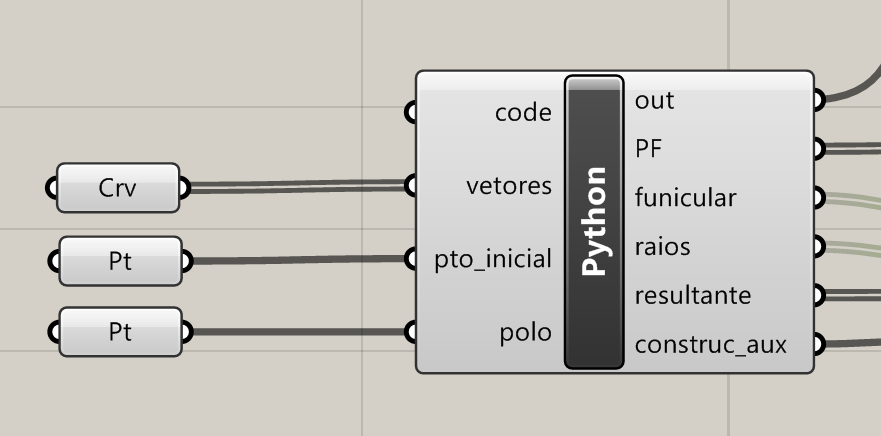
\includegraphics[width=.75\textwidth]{Algfunicular01B.png}
\caption{Entradas e sa�das do componente} \label{figura:Ap1:Algfunicular01B}
\end{center}
\end{figure}

V�deo registrando o funcionamento do algoritmo dispon�vel em:

\href{https://www.youtube.com/watch?v=pIa0o2M0-_s}{https://www.youtube.com/watch?v=pIa0o2M0-\_s}

